% Author: Joel Scarinius Stävmo, Oskar Sundberg, Linus Savinainen, Samuel Wallander Leyonberg  and Gustav Pråmell
% Update: October 1, 2024
% Version: 1.0.0
% License: Apache 2.0

A Genetic Algorithm Based Elevator Dispatching Method For Waiting Time Optimization \cite{tartan2016genetic} explains how they solve a similar problem but with multiple elevators \( what they call cars \) instead this paper only looks at one elevator per building. This paper has been the starting point in terms of algorithms and approaches this report. This by following their flow chart provided in the paper, see Figure 1. 

\begin{figure}[ht]
\centering
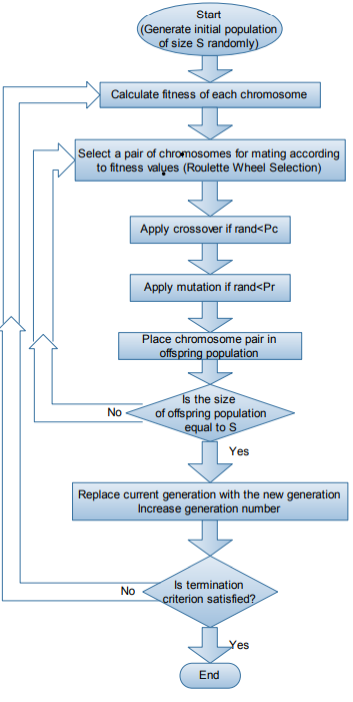
\includegraphics[width=0.4\textwidth]{diagram_1.png}
\caption{From ..}
	\label{fig:Flow_1}
\end{figure}
The paper describes a 21\% improvement with their methods compared to Ghareib paper \cite{gharieb2005optimal} on the same problem. As this problem is not interlay equal to ours, comparison with this would not give a representee outcome. However, by following the approach in the paper simulations were run for the problem space and compare the results to results given with \( theoretically \) more suited genetic operations.
\newpage

\begin{figure}[ht]
\centering
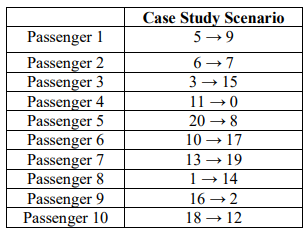
\includegraphics[width=0.4\textwidth]{tabel_1.png}
	\label{fig:Tabel_1}
\caption{From ..}
\end{figure}

\cite{ahmed2022investigation} investigates for different approaches in terms of algorithm to the problem at hand.  One of there algorithm to solve the elevator dispatching problem is a genetic algorithm where they use Davis-order crossover, swap mutation and calculate average time for occupants  witch is used as fitness function. There building \( problem space \) and predefined settings where as following:

The results from their test show that GA where the best performing algorithm for this problem with the definitions above.

This paper presents results that we later compare to ours with our first implementation as given of the flow chart \cite{tartan2016genetic} as well as later implementation with updated genetic operations. Given their result for testing different algorithms on the problem, a genetic algorithm approach seems to contribute with the best result to the elevator dispatching problem.

Crossover and Mutation Operators of Genetic Algorithms \cite{lim2017crossover} lists and shortly describes different types of crossover and mutation operations. They describe Wright's heuristic crossover and categorized it as one of the crossover functions how’s offspring are “in the exploration region near the parents” \cite{lim2017crossover} . This reduce premature offspring by overcoming local maximum. On further investigation into different implementations of heuristic crossover, the concept seamed as a good crossover function for the reports problem due to its simplicity and ability to be largely modified to suit the reports problem and fitness function.


